\documentclass[a4paper,11pt]{article}
\usepackage[osf]{mathpazo}
\usepackage{ms}
\usepackage[]{natbib}
\raggedright

\newcommand{\plant}{\texttt{plant}}
\newcommand{\smurl}[1]{{\footnotesize\url{#1}}}
\usepackage{graphicx}

\title{{\plant}: A package for modelling forest trait ecology \& evolution}
\author{Daniel S. Falster\textdagger\textasteriskcentered$^1$, Richard G. FitzJohn\textdagger$^1$, \\{\AA}ke Br{\"a}nnstr{\"o}m$^{2,3}$, Ulf Dieckmann$^3$, Mark Westoby$^1$}
\affiliation{
$^1$ Department of Biological Sciences, Macquarie University, Sydney, NSW 2109, Australia\\
$^2$ Department of Mathematics and Mathematical Statistics, Ume{\aa} University, 901 87 Ume{\aa}, Sweden \\
$^3$ Evolution and Ecology Program, International Institute for Applied Systems Analysis, Schlossplatz 1, A-2361 Laxenburg, Austria \\
\textdagger These authors contributed equally.\\
\textasteriskcentered Email for correspondence: \texttt{daniel.falster@mq.edu.au}\\
A manuscript in consideration as an Applications Note for
publication in MEE as part of the Special Feature \emph{Demography
 beyond the Population}.\\
Word count: ~4200 words}
\date{}

\bibliographystyle{mee}

\usepackage[title,titletoc,toc]{appendix}

\mstype{Applications Note}
\runninghead{The {\plant} package}
\keywords{demography, emergent, fitness, growth,
physiology, metapopulation, mortality, reproduction, size-structure,
tradeoff}

\begin{document}
\mstitlepage
\noindent
\parindent=1.5em
\addtolength{\parskip}{.3em}
\doublespacing
\linenumbers
\section{Summary}\label{abstract}
\begin{enumerate}
\def\labelenumi{\arabic{enumi}.}
\itemsep1pt\parskip0pt\parsep0pt
\item
 Population dynamics in forests are strongly size-structured:
 larger plants shade smaller plants while also expending
 proportionately more energy on building and maintaining woody stems.
 Although the importance of size
 structure for demography is widely recognised, many models
 either omit it entirely, or include only coarse approximations.
\item
 Here we introduce the {\plant} package, an
 extensible framework for modelling size- and trait-structured demography,
 ecology and evolution in simulated forests.
 At its core, {\plant} is an
 individual-based model where plant physiology and demography are mediated by
 traits. Individual plants from multiple species can be grown in isolation,
 in patches of competing plants, or in metapopulations under a
 disturbance regime.
 These dynamics can be integrated into metapopulation--level
 estimates of
 invasion fitness and vegetation structure. Because fitness emerges as a
 function of traits, {\plant}
 provides a novel arena for exploring eco-evolutionary dynamics.
\item
 {\plant} is an open source R package and is available at
 \href{https://github.com/traitecoevo/plant}{github.com/traitecoevo/plant}.
 Accessed from R, the core routines in {\plant} are written in C++.
 The package provides for alternative physiologies and for
 capturing trade-offs among parameters. A
 detailed test suite is provided to ensure correct behaviour of the code.
\item
 {\plant} provides a transparent platform for investigating how
 physiological rules and functional trade-offs interact with competition and
 disturbance regimes to influence vegetation demography, structure and
 diversity.
\end{enumerate}

\section{Introduction}\label{introduction}

Plant growth and demography are fundamentally size- and
trait-structured, influencing dynamics over time-scales ranging from
instantaneous physiological effects to long-term evolutionary outcomes
\citep{Harper-1977, Westoby-2002, Griffith-2016, Rees-2016}.
%
As an individual plant increases its leaf area, it increases its potential
to generate photosynthate.
%
On the other hand, as individuals grow larger, they must allocate increasing
fractions of their photosynthetic income to activities other
than building new leaves; for example, to maintaining support tissues
\citep{Givnish-1988, Enquist-2007} or to reproduction
\citep{Thomas-2011}.
%
Consequently, rates of growth, mortality and reproduction change with
individual size \citep{Muller-2006, Ruger-2011, Thomas-2011}.
Ontogenetic
patterns of growth also vary with traits; for example,
leaf and wood construction costs influence growth rates
\citep{Falster-2011, Visser-2016}, while seed size and height
at maturation determine start and end points of ontogenetic
trajectories \citep{Westoby-2002}.
%
Strong feedbacks emerge between individuals within a forest via
competition for light and other resources, such that the growth rate
of one individual depends on the size and traits of nearby
individuals \citep{Shugart-1980, Pacala-1996}.
%
Such feedbacks make it difficult to link observable species traits to
phenomena such as self-thinning, successional transitions, trait
evolution and species coexistence, without
modelling both individual growth and the competitive interactions between
individuals.

Although the importance of size structure for trait evolution, vegetation
dynamics and diversity has long been recognised \citep[e.g.,][]{Harper-1977,
 Shugart-1980, Huston-1987}, current research in this area is
dominated by models and theory that either omit size structure
entirely, or only include coarse approximations.
%
Theoretical investigations exploring questions about niche-based
species coexistence and ecological drift (neutrality) both rely
primarily on unstructured population models \citep[e.g.,][]{MacArthur-1967,
 Tilman-1985, Geritz-1998, Hubbell-2001, Calcagno-2006}.
%
It is common to assume competitive outcomes to be influenced by
size-related traits such as adult size and seed size, but detailed
size structure is rarely considered, at least in plant models
\cite[for animal examples, see][]{Deroos-1997}.
%
Similarly, many of the models used to study global vegetation dynamics across
the last 20 years have not included size-structured demography
\citep[for comparisons of some major models, see][]{Sitch-2008,
Dekauwe-2014}.
%
While the importance of explicitly including size-structured dynamics is
increasingly recognised in both evolutionary ecology
\citep[e.g.,][]{Falster-2015, Rees-2016} and vegetation dynamics
\citep[e.g.,][]{Moorcroft-2001, Purves-2008, Smith-2014,
Weng-2015, Sakschewski-2015}, our understanding of how these features
impact the ecology and evolution of vegetation communities remains
relatively limited.

In this note, we introduce the {\plant} package for R \citep{R-2015};
a framework for studying the effects of size structure and
trait variation on the demography of individual plants, of patches of
competing plants and of metapopulations structured by a
disturbance regime.
%
Our own purpose in developing {\plant} has been mainly to investigate how species
differing in traits may be able to coexist with one another
\citep[following ][]{Falster-2011, Falster-2015}; as size-structured models
provide unique opportunities for studying coexistence via differentiation in
successional strategy \citep[see also][]{Huston-1987, Moorcroft-2001, Uriate-2016}.
At the same time, we expect {\plant} to be useful for modelling other demographic and evolutionary phenomena.

Broadly, the {\plant} package falls into a class we refer to as trait-, size- and
patch-structured models \citep[\textsc{TSPMs}, following][]{Falster-2011}. \textsc{TSPMs} are direct
descendants from the ``gap'' models developed in the 1980s
\citep[e.g.,][]{Shugart-1980, Huston-1987, Kohyama-1993}; other modern examples
include \textsc{ED} \citep{Moorcroft-2001}, \textsc{LPJ- GUESS}
\citep{Smith-2014} and \textsc{LPJmL-FIT} \citep{Sakschewski-2015}. Common to
\textsc{TSPMs} is that they explicitly model size-structured competition
among individual plants within a metapopulation of ``patches'', where
individuals can differ in their traits and thus demographic behaviour.
\textsc {TSPMs} typically ignore the spatial structure of plants within
patches and the spatial structure of patches relative to one another. Instead,
they focus computational effort on resolving the dynamics of size-structured
competition for light and successional turnover. Differences among
\textsc{TSPMs} arise from the core physiological models used (describing
how the demography of individual plants responds to resource availability),
and also from the numerical techniques applied to scaling the physiological model
up to estimate emergent behaviours of individuals, patches and vegetation.

Below we describe the general approach of the {\plant} package, then provide
sections outlining potential applications at nested levels of ecological organisation.
More detailed technical documents are provided as supplementary information
(see Appendices; updated versions of these technical documents are
available within the {\plant} package itself). These documents outline \ref{sec:demography}) the system of
equations being solved when modelling the demography of plants, patches and metapopulations; \ref{sec:FF16}) a description of the core
physiological model used in {\plant}, and \ref{sec:code}) a compendium of worked code examples showing how to interact with the {\plant} package from R.

\section{Overview of approach}

The {\plant} package implements an individual-based model, meaning that the dynamics of the
population arise from rules specifying how individuals grow and interact.
Being driven by traits, the model can be extended to potentially very many species. The
core rules in {\plant} are about the short-term physiological
functioning of an individual plant and how this is influenced by its
traits, size and light environment. While {\plant} includes a core physiological model, the present paper uses it only as an example, to illustrate how one can take a given physiological model and simulate ecological and evolutionary outcomes. Thus, we do not aim to justify the particular physiological model used, to provide detailed
comparisons to data, or to promote this physiological model over those
in other \textsc{TSPMs}. (These are all topics deserving substantially
more attention than can be afforded here.)
An important feature of {\plant} considered as a software package is that it allows for users to substitute their own physiological models.

On top of the physiological model, {\plant} implements methods for
population dynamics and adaptive dynamics (Fig. \ref{fig:schematic}), following methods
described by \citet{Falster-2011} and \citet{Falster-2015}. Demographic
phenomena can be studied at three levels: individual plants, stands of
competing plants and entire metapopulations. The dynamics at higher
levels of organisation arise as emergent properties, driven by growth
physiology, competition for light and disturbance (Fig. \ref{fig:schematic}).
{\plant} offers the capacity to model emergent phenomena in patches with
specified area, and also through a deterministic approximation
where specifying a patch size is not required. Trait evolution and community
assembly can then be modelled using the estimates of invasion fitness
provided by {\plant}.

\section{Effects of size, trait and light environment on the demography of individual plants}

The core of {\plant} is a model for an individual species' physiological
strategy as specified by its traits (Fig. \ref{fig:schematic}a). For
present purposes, a species is defined as a group of individuals with identical
traits. The effects of trait variation is to modify parameters of the core
physiological model, which in turn translate into different demographic outcomes.

The default physiological model used in {\plant} largely reflects
that presented in \citet{Falster-2011, Falster-2015}, but with extensions
allowing for growth in plant diameters also to be estimated. We refer to this
default model as \texttt{FF16}, reflecting the initials of the first two authors
and publication year of this paper. The \texttt{FF16} model estimates rate
of biomass
production for a plant, given its size and the current light
environment. Gross photosynthetic income is calculated from the total
leaf area and the light distribution across the plant's canopy. Costs
of tissue respiration and turnover are subtracted. The remaining
biomass production is allocated between growth and reproduction. The key
outputs needed by higher levels of {\plant} are height
growth rate, mortality rate and rate of seed production (Fig. \ref{fig:schematic}). Additional quantities are also computed, such as total assimilation, as well as
respiration, turnover and allocation rates for different
tissues; these intermediates can also be accessed (for further details on the \texttt{FF16} model, see Appendices
\ref{sec:FF16} and \ref{sec:code}).

While we have implemented a particular physiological model
(\texttt{FF16}), the package is designed to allow arbitrary
additional physiologies to be introduced. Users are able to modify the
physiological model in three different ways. First, one can vary the
parameters of the \texttt{FF16} model directly (see Appendix
\ref{sec:FF16} for the list of parameters and Appendix \ref{sec:code} for code
examples). Second, we allow for changes in key parameters to bring
about changes in other parameters (a hyper-parameterisation), enabling the
straightforward modelling of trade-offs. For example, the
trait \textsc{lma} (leaf mass per unit leaf area) is used by default to estimate
the rate of leaf turnover ($k_{\rm l}$), based on an observed scaling
relationship spanning across diverse vegetation and plant functional
types \citep{Wright-2004},
$$k_{\rm l} = \beta_{{\rm kl}1} \, \left(\phi / \phi_0\right)^{-\beta_{{\rm kl}2}},$$
where $k_{\rm l}$ and $\phi$ (\textsc{lma}) are both parameters of the core physiological
model, and $\beta_{{\rm kl}1}, \beta_{{\rm kl}2}, \phi_0$ are hyper-parameters. Such
linkages are defined within a user-supplied hyper-parameterisation function
(see Appendix \ref{sec:FF16} for details, or Appendix
\ref{sec:code} for code examples).
%
Finally, rather than varying the parameters of the existing equations
in the \texttt{FF16} model, the equations themselves can be
fundamentally changed. This requires defining a new physiological
model in a new C++ file and compiling that into the package. As an
example, in the \texttt{FF16R} physiology, we have shown how to modify the
function determining allocation to reproduction.

With a physiological model in place, {\plant} can be used to estimate
essential physiological rates for individual plants
(Fig. \ref{fig:plant}). The function \texttt{grow\_plant\_to\_size}
takes a given strategy and light environment and grows the plant,
producing a trajectory of plant size over time (Fig. \ref{fig:plant}a). This
is achieved by integrating an ordinary differential equation with a
size-dependent growth rate (see Appendices \ref{sec:demography} and
\ref{sec:code} for details). As the plant grows, allocation to
different tissue types varies; specifically, the composition of the plant
changes to include more stem and less leaf
(Fig. \ref{fig:plant}b). This, in turn, affects maintenance and turnover
costs and the growth rate of the plant. By itself, the
shift in allocation can generate the widely observed hump-shaped dependence
of absolute height growth on plant height \citep[Fig. \ref{fig:plant}c;][]{King-2011}, as well as the decline in relative mass growth rate with plant size from birth onwards \citep{Enquist-2007}.

By varying the light environment and measuring growth rate, the whole-plant light compensation point (\textsc{wplcp}) can be computed (Fig.
\ref{fig:plant}d). The \textsc{wplcp} is the light level where the plant
stops growing, increasingly regarded as the most useful
measure of a species' shade tolerance
\citep{Givnish-1988, Baltzer-2007, Lusk-2013}. As expected, the \textsc{wplcp}
increases with plant size (Fig. \ref{fig:plant}d), due to increased costs of building and
maintaining stem and leaf tissues \citep{Givnish-1988}. Likewise, the \textsc{wplcp}
decreases with \textsc{lma} (Fig. \ref{fig:plant}d), because high-\textsc{lma} species have slower leaf turnover \citep{Baltzer-2007, Lusk-2013}.

\section{Plants competing in a patch}

Within patches of competing plants, competition for light generates
strong nonlinear feedbacks on growth, survival and reproduction. In the
\texttt{FF16} physiological model, we consider only the effects of
shading on rates of biomass production. Competition for other
resources such as nitrogen or water could be considered by extending the
physiological model. We assume that patches are vertically -- but not horizontally --
structured; in other words, we account for size differences, but not for the spatial
layout within patches. Similar assumptions are made in other \textsc{TSPMs}
\citep{Shugart-1980, Kohyama-1993, Huston-1987, Moorcroft-2001, Smith-2014}, and also
in related approaches, such as Integral Projection Models \citep[e.g.,][]{Rees-2016}.
While one would ideally also consider spatial interactions within patches,
such models are very computationally demanding \citep{Shugart-1980,
Pacala-1996}. Simplifying spatial interactions within patches can be motivated from the observation
that competitive thinning tends to break down spatial clusters
\citep{Strigul-2008}.

When modelling a patch of competing plants, the focus is on how the size distribution \(N(H | x, a)\) changes with patch age \(a\), with the latter defined as the time that has passed since the last disturbance. This distribution describes the density \(N\) of
individuals with height \(H\) for given traits \(x\) and patch age \(a\).
The density \(N\) is measured as individuals per unit height and per unit ground area.
Modelling the dynamics of \(N(H | x, a)\) requires that both the initial size distribution and the inflow of new recruits be specified. We have primarily
been interested in the dynamics of a patch recovering from disturbance and have
therefore started with an empty patch and a constant flow of seeds from a global
seed rain (Fig. \ref{fig:schematic}b). A (non-trivial) extension would result from allowing some plants to survive disturbance \citep[following][]{Kohyama-1993}.

{\plant} offers two methods for modelling the dynamics of \(N(H | x, a)\)
in a competing population. In the first stochastic mode, users
specify an average seed rain and patch size, and {\plant} then generates a
vector of seed arrival events and simulates the stochastic
development of the resulting finite-sized population.

For most applications, however, rather than modelling
dynamics within a finite-sized stochastic patch, it will be preferable to use {\plant}'s
deterministic mode. This assumes that
patches are sufficiently large that population dynamics within a
patch approach their deterministic limit and can
be approximated via a physiologically structured population model \citep{Metz-1986, Deroos-1997, Kohyama-1993}. These models are often formulated as partial differential equations where boundary conditions and coefficients may depend on the population state. Such structured population models are also thought to
capture the average behaviour across a large number of small patches
\citep{Moorcroft-2001}. Importantly, the deterministic mode in {\plant} is
much faster than the stochastic mode, and eliminates the demographic noise
that inevitably arises in finite-sized populations (see Appendix \ref{sec:demography} for details).

Our approach for numerically solving deterministic size-structured population dynamics is
based on the characteristic method \citep{Angulo-2004}. This method describes the development of
the size distribution\(N\) by approximating it along a collection of individual growth trajectories spanning the size
spectrum. Following a disturbance, a series of such trajectories are introduced
into each patch. These trajectories then change according to the growth
of the corresponding individuals, conditioned on their survival
(Fig. \ref{fig:patch}a). Meanwhile, growth and mortality combine
to alter the density of individuals along these trajectories
(Fig. \ref{fig:patch}b). The characteristic method is similar to the Escalator Boxcar Train (\textsc{EBT})method
\citep{Deroos-1997} used by \citet{Falster-2011} and
\citet{Falster-2015}, but not identical. An advantage of the characteristic method is that it allows direct approximation of the size distribution. For the same reason, however, the characteristic method may be less suitable for resolving size distributions in models where those distributions naturally develop sharp peaks (which happens, e.g., when plants completely cease to grow at a given height).

We implement a novel technique for
handling strongly size-asymmetric competitive feedbacks, such as those occurring
under strong competition for light (see Appendix \ref{sec:demography}
for details). This technique works for both the characteristic method and the \textsc{EBT} method. It involves an
adaptive refinement of the time points where new growth trajectories or cohorts are introduced
into the population, an idea first applied in \citet{Falster-2011} and
described further in \citet{Falster-2015}.
Normally, growth trajectories are introduced evenly, spaced out according to a fixed time
interval. Under size-asymmetric competition, however, the growth
trajectories of individuals born at nearby times can diverge
substantially over time (Fig. \ref{fig:patch}a; Appendix
\ref{sec:demography} and \ref{sec:code}). This can become a problem during patch
development, because much of the population can be located in between
widely-spaced trajectories, causing low numerical accuracy. To maintain
numerical accuracy, we use an iterative algorithm to adaptively refine
the cohort spacing until adjacent trajectories remain
adequately resolved throughout patch development (see Appendix
\ref{sec:demography} for details). This refinement gives rise to an uneven
distribution of cohort introduction times across patch age (Fig.
\ref{fig:patch}a), with a considerably tighter spacing of trajectories in
younger patches.

Modelling the full size-structured dynamics within patches enables multiple demographic phenomena to be
investigated. First, {\plant} can simulate demographic
phenomena typically observed in patches
recovering from a disturbance, including self-thinning and
successional replacement. Whereas other approaches for modelling
self-thinning are limited to a single species
\citep[e.g.,][]{Barnes-2004, Coomes-2007}, \textsc{TSPMs} can accommodate
multiple species with different traits (Fig. \ref{fig:schematic}b;
Fig. \ref{fig:patch}). Second, the self-thinning and
successional replacement emerges from the
combined effects of physiology and competition for resources, rather
than being prescribed by the model. As a consequence, it is possible to ask how alternative trait values affect fitness (see below). Third, \textsc{TSPMs} allow the combined effects of physiology and succession on a patch's emergent
properties to be investigated
\citep{Moorcroft-2001, Falster-2011}. In particular, leaf area cover and rates of biomass
production tend to vary nonlinearly with patch
age \citep{Smith-2001, Binkley-2002, Ogawa-2010};
in {\plant}, such outcomes naturally arise as emergent properties,
driven by underlying physiology and demography (Fig. \ref{fig:patch}c).

\section{Trait-, size- and patch-structured vegetation}

All vegetation in {\plant} is subject to a disturbance regime, implying that patches
are cleared at a given rate \citep[e.g.,][this issue]{Treurnicht-2016}.
Such clearance can be interpreted, for example
as resulting from a fire, cyclone, clear-cutting or
landslide. The vegetation thus comprises a series of patches
differing in the time that has passed since their last disturbance, linked via seed dispersal
(Fig. \ref{fig:schematic}b). Such a system is often referred to as a
structured metapopulation \citep{Gyllenberg-2001}.

In {\plant}, following an approach established in previous \textsc{TSPMs}
\citep{Kohyama-1993, Moorcroft-2001, Falster-2011},
we assume an infinite number of patches, all experiencing
the same disturbance regime and sharing a common seed dispersal pool, or global seed rain
(as in the island model; Fig. \ref{fig:schematic}b). As mentioned before, we also assume
that disturbances remove all vegetation. With this
approach, we can scale up from deterministically solving the dynamics of
a single patch to solving the dynamics of an entire metapopulation.
Under these assumptions, the frequency distribution \(P(a)\) of patches aged
\(a\) changes deterministically according to a second partial differential equation (see Appendix
\ref{sec:demography} for details). The scaling from patches to the
metapopulation is then achieved by weighting the temporal dynamics of
a single patch by \(P(a)\), i.e., by the relative abundance of patches aged
\(a\) in the metapopulation (Fig. \ref{fig:patch}c).

The main numerical challenge in stepping from a single patch to a
metapopulation is to identify the equilibrium seed rain of the
metapopulation. An input seed rain is required to simulate the
demography of the metapopulation, and this in turn produces an output
seed rain. Equilibrium occurs when, for each species,
the input seed rain equals the output seed rain. Identifying this equilibrium
requires finding the root of a multi-dimensional function, subject to
the constraint that a unique positive root exists and the root is dynamically stable (the trivial equilibrium
of zero seed rain always exists, but is often not stable; Appendix
\ref{sec:code}). Solving for multi-dimensional roots can be computationally challenging,
with no single technique guaranteed to find a solution. In {\plant}, we sequentially
apply rounds of iteration and nonlinear root finding, while also
using some heuristics to try to ensure that the root returned is an attracting point
(see Appendix \ref{sec:demography}, \ref{sec:code} for details). Real seed rains are of course noisy,
but the aforementioned approach allows for mean tendencies to be estimated (which is required for computing fitness; see below).

An attractive feature of the metapopulation concept implemented in \textsc{TSPMs}
is that it integrates equilibrium and non-equilibrium approaches to
modelling ecological dynamics \citep{Kohyama-1993, Moorcroft-2001,
 Falster-2011}. An equilibrium being approached at the level of
the metapopulation implies that seed rain and size structure across the
metapopulation are approximately stable. Yet, even under this condition, the structure of
vegetation within individual patches remains constantly in flux: patches
continue to age, and their residents continue to grow, until the next disturbance occurs.

Such dynamic equilibria arising in \textsc{TSPMs} potentially resolve several
challenges faced by unstructured models. First, by scaling up from
patches to a metapopulation, we close the demographic feedback loop and
create a self-regulating system. {\plant} yields as outputs the equilibrium seed rains and size distributions for each considered species, based on the combined effects of the model's physiological rules, species traits, competitive interactions
and disturbance regime.

Second, the metapopulation concept allows for the effects of disturbance
regimes on vegetation structure and dynamics to be properly incorporated. In
{\plant}, characteristics for the entire vegetation (metapopulation) -- such
as total leaf area, biomass and productivity -- are obtained by averaging
patch-level outcomes over the frequency distribution of patch ages (e.g.,
Fig. \ref{fig:patch}c). Similarly, the distributions of abundance and growth rate
observed in large forest plots \citep[e.g.,][]{Muller-2006, Coomes-2007} arise
as emergent properties. Moreover, the predictions from {\plant}
are for a frequency distribution of patch states across the landscape
(Fig. \ref{fig:emergent}, see Appendix \ref{sec:code} for details). As such,
size- and patch-structured models provide unique opportunities for linking with
satellite data and forest survey data \citep{Moorcroft-2001, Purves-2008}.

Finally, with the extension to the metapopulation level, we are
modelling demography across the entire plant life cycle and are thus in a
position to estimate invasion fitness -- the rate at which a rare
individual with particular traits can establish (positive invasion fitness) or cannot establish (negative invasion fitness) in a community of
established residents at their equilibrium densities
\citep{Metz-1992}. While often calculated as the
long-term per capita growth rate, a more convenient indicator of
fitness in structured metapopulations is given by the
logarithm of the basic reproduction ratio, \(R\) \citep{Gyllenberg-2001, Metz-2001}. The basic reproduction ratio is simply the average number of seeds produced from one seed of a new type over its lifetime, averaged across the metapopulation. So a new type can
invade when \(R > 1\). The calculation of \(R\) available in
{\plant} follows equations given by \citet{Falster-2015}
(see Appendix \ref{sec:demography} for details).

With this measure of fitness, we can model trait-based adaptive
dynamics, and community assembly \citep{Metz-1992, Geritz-1998,
Chesson-2000, Dieckmann-2004, Brannstrom-2013b}. An example
for forests was introduced by
\citet{Falster-2015}. This is best thought of as occurring on a fitness landscape,
a surface with fitness plotted against one or more traits
(Fig. \ref{fig:fitness}). The reproductive success of individuals
depends both on their own traits and on the densities of other occupants in the current resident community. Fitness landscapes are positive in trait regions that allow invasion, and zero
for resident species that are at equilibrium. The slope of the fitness
landscape with respect to traits determines the direction of selection,
for example the negative slope of the dashed line around the resident
in Fig. \ref{fig:fitness}a)indicates selection for
smaller trait values (see Appendix \ref{sec:code} for
details). Fitness landscapes are continually reshaped as species are
introduced and their trait values evolve, reflecting the nonlinear demographic feedbacks
that occur under frequency-dependent evolution. Stable coexistence is
possible when species with different traits can mutually invade.
Following the fitness gradient may lead to an
evolutionary branching point; at
such a point, there is no directional selection (solid line in
Fig. \ref{fig:fitness}a), but both smaller and larger trait values can invade.
It is often possible to find a species configuration where
fitness is negative everywhere (solid line in Fig. \ref{fig:fitness}b)
except for the zero points where species are present. Such communities
are immune to invasions by species with any other trait values and represent
predictions for the trait mixtures favoured by
natural selection .

Identifying conditions promoting trait diversity is a valuable role
for {\plant}. The simple example shown in the present paper can be extended to multiple dimensions
and can be used to investigate how trade-offs facilitate coexistence
\citep{Falster-2015}. Co-occurring plant species differ in a range of physiological
traits, yet the conditions allowing for stable coexistence remain largely
unknown \citep{Adler-2013}.
A variety of algorithms from the area of adaptive dynamics theory can be
applied for modelling community assembly \citep[e.g.,][Fig. \ref{fig:schematic}]{
Geritz-1998, Dieckmann-2004, Brannstrom-2013b, Falster-2015}, using the estimate of invasion fitness provided by {\plant}.

\section{Implementation details}

{\plant} is written in C++ and R, using the packages \texttt{Rcpp}
\citep{Eddelbuettel-2011, Eddelbuettel-2013} and \texttt{RcppR6}
\citep{RcppR6} to bridge between the two languages. Due to the
computationally intensive nature of the model, the core physiological
and demographic components are written in C++ to maximise speed. We used
templated types that allow the demographic and evolutionary components
to be driven by alternative physiological models while retaining the
same interface at higher levels. Despite mostly being written in C++,
all components of the model, down to individual plants, can be
extracted and interacted with dynamically in R.

{\plant} makes use of much existing software, including the R
computational environment \citep{R-2015}, the R packages \texttt{Rcpp}
\citep{Eddelbuettel-2011, Eddelbuettel-2013}, \texttt{R6}
\citep{Chang-2014}, and the Boost Library for C++
\citep{Schaling-2014} via the R package \texttt{BH}
\citep{Eddelbuettel-2015}. Source code is hosted at
\href{https://github.com/traitecoevo/plant}{github.com/traitecoevo/plant}.
Installation instructions are available at this webpage, and binary
releases will also be available there. ({\plant} does not
currently compile on Windows, but this will change as soon as R core
upgrade the Windows C++ compiler.)

\section{Comparison with existing software}

Increased interest in capturing the dynamics of size-structured populations
\citep[e.g.][]{Griffith-2016}
has prompted development of several tools, each with its own distinct
strengths. The \textsc{EBT} software \citep{Deroos-1997}, {\plant} is customised for plants, and
to that end offers refinements needed to handle modelling of the strongly
size-asymmetric feedbacks that occur in plant communities, as well as the
extension to a structured metapopulation. Other \textsc{TSPMs} also exist for modelling of vegetation, like \textsc{ED}
\citep[ver 1 and 2;][]{Moorcroft-2001, Medvigy-2009}, \textsc {LPJ-GUESS}
\citep{Smith-2014} and \textsc{LPJmL-FIT} \citep{Sakschewski-2015}. These
models were designed for simulating bio-geochemical cycles and vegetation
structure across broad geographic areas, and their architectures are
optimised for such use. By contrast, {\plant} was designed so that the
physiological rules driving the dynamics of the system could be easily
manipulated and emergent demographic properties (including those of individual plants, patches, metapopulations of patches and fitness) studied in
detail. Finally, like {\plant}, the \textsc{LM3-PPA} \cite{Weng-2015} model also aims
to scale from individual-level processes to emergent properties of
vegetation, including estimating invasion fitness. Yet the approaches taken
for solving the dynamics are very different. The \textsc{LM3-PPA} relies on
complex analytical solutions to the size-structured interactions, whose
derivation required simplifying elements of the physiology and ecology in that
model. By contrast, in {\plant} we have retained the full range of
physiological and ecological feedbacks, and instead relied on using robust
numerical methods to solve the system dynamics (see Appendix
\ref{sec:demography} for details).

\section{Closing comments}

The {\plant} package is designed to make it easier for researchers and forest
practitioners alike to investigate a variety of nonlinear demographic, ecological and evolutionary
phenomena. Rather than provide a model with a few entry points, we
have developed an extensible framework that we hope can be used to
answer a number of questions at a variety of scales. The specific
applications highlighted here arise from our interest in the assembly of
trait mixtures in communities. A variety of other uses are
possible, addressing other aspects of community assembly and function. For
example, we expect the package will prove useful for i) investigating
how morphological and physiological traits influence growth rate and
shade tolerance, ii) studying emergent phenomena such as multi-species self-thinning, successional transitions and age-related changes in
vegetation productivity, and iii) bridging between empirical data,
large-scale simulators of global biogeochemical cycles and simple
abstract theoretical models.

\section{Acknowledgements}

We thank J Camac, A De Roos, R Duursma, J Johansson and C Prentice for helpful
discussions and three anonymous reviewers for comments on an earlier draft. Falster
was supported by an Australian Research Council (ARC) discovery grant (DP110102086).
FitzJohn was supported by the Science and Industry Endowment Fund (RP04-174).
Br{\"a}nnstr{\"o}m was supported by the Swedish Research Council Formas (2012-2008).
Dieckmann was supported by the European Commission, the European Science Foundation,
the Austrian Science Fund, the Austrian Ministry of Science and Research, and the
Vienna Science and Technology Fund. Westoby was supported by a fellowship from the ARC.
The authors have no conflicts of interest to declare.

\section{Data Accessibility and Reproducibility}

Source code for reproducing the entire contents of this paper is available at
\href{https://github.com/traitecoevo/plant\_paper}{github.com/traitecoevo/plant\_paper};
see also Appendix \ref{sec:code} for worked examples reproducing the figures.
This paper does use any data.

\section{Author contribution statement}

RGF and DSF wrote and developed the software, including numerical algorithms. AB and UD helped develop algorithms included in prototype software. DSF, RGF and MW wrote the the paper, with input from AB and UD. All authors contributed to material presented in Supplementary material.

\clearpage
\bibliography{refs}

\clearpage

\section{Figures}\label{figures}

\begin{figure}[h!]
\centering
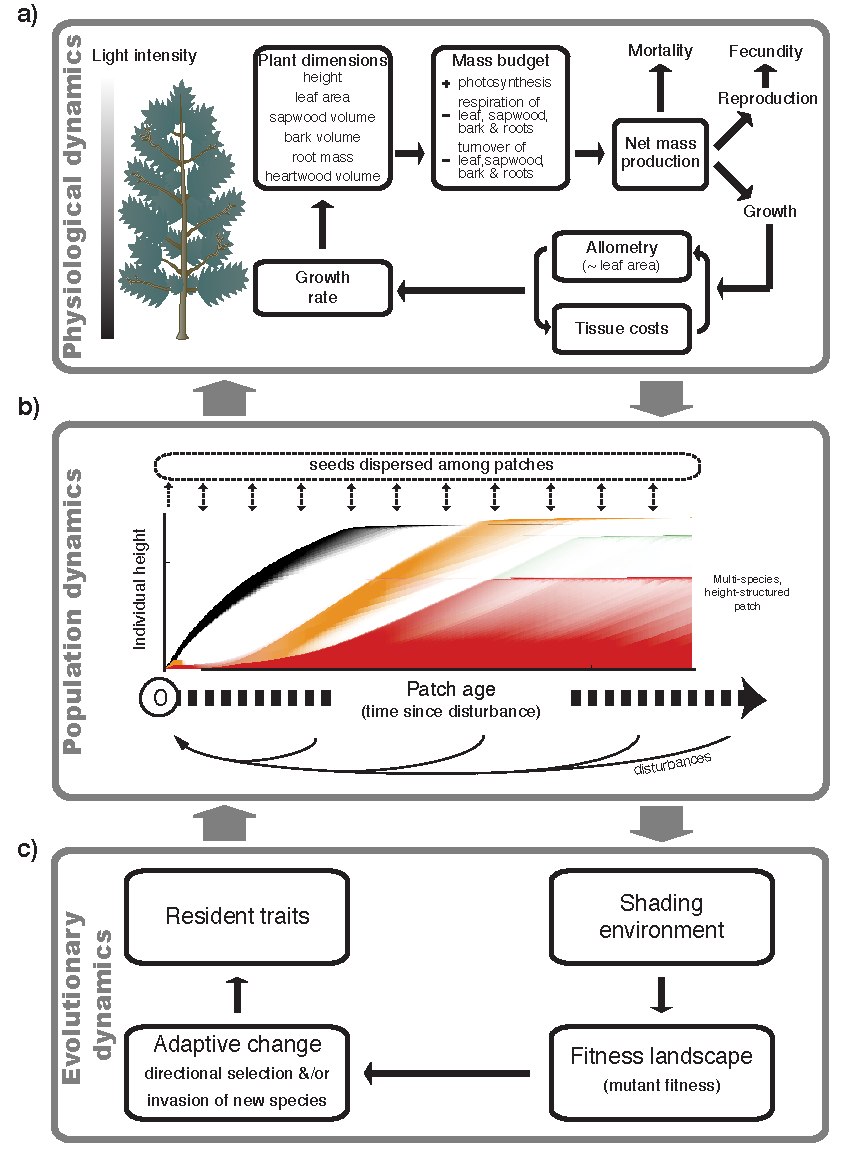
\includegraphics[width=15cm,height=15cm,keepaspectratio]{figures/schematic}

\caption{Processes modelled within {\plant} include physiological, population and
adaptive dynamics.
(a) Dynamics across all three levels are driven by the
physiological sub-model determining an individual's physiological and
demographic rates on the basis of its traits, size and light environment.
(b) Competitive hierarchies are modelled by tracking the height distribution of
individuals within a patch. The intensity
of shading indicates the density of individuals at a given height for
different species (distinguished by colours). A size- and patch-structured
metapopulation consists of a distribution of patches linked by a global seed rain.
Disturbances occasionally remove all vegetation within a patch, resetting its vegetation. (c) The traits of the resident species determine the light environment
in all patches across the metapopulation, which in turn determines the invasion fitness.
The dashed outline indicates that users must supply their own algorithms for
modelling trait evolution and community assembly, using the estimate of
invasion fitness provided by {\plant}. Figure adapted from
\citet{Falster-2011}, \citet{Falster-2015}.
}

\label{fig:schematic}
\end{figure}

\newpage

\begin{figure}[h!]
\centering
\includegraphics[width=15cm,height=15cm,keepaspectratio]{figures/plant.pdf}
\caption{Physiological dynamics for individual plants varying in size,
 trait and light environment. Solid lines refer to the high-\textsc{lma} (leaf mass per unit leaf area) strategy (\textsc{lma} =
 0.2625), while dashed lines refer to the low-\textsc{lma} strategy
 (\textsc{lma} = 0.0825). (a) Growth trajectories are influenced by
 both light environment and traits. (b) Over time, the fraction of
 living tissue switches from leaf towards sapwood, with high-\textsc{lma} species having relatively more mass in leaf than low-\textsc{lma} species. (c)
 Size-dependent height growth rates, being the derivatives of the functions in (a), peak at a height of around
 5m, but the location of this peak varies with both trait and light
 level. (d) Declines in height growth rate with light level vary with plant size
 and traits. Whole-plant light compensation points (indicated by
 circles) emerge at zero growth rate (intercepts on horizontal axis).
 The light level used in (a) and (c) is indicated by
 coloured ticks. See Appendix \ref{sec:code} for code
 reproducing this figure.}
\label{fig:plant}
\end{figure}

\newpage

\begin{figure}[h!]
\centering
\includegraphics[width=15cm,height=15cm,keepaspectratio]{figures/patch.pdf}
\caption{Population dynamics for two species competing within a patch.
 Red and blue lines refer to the low- and high-\textsc{lma} species from
 Fig. \ref{fig:plant}. (a) Growth trajectories
 for individuals germinating across a range of patch ages for each
 species, using a schedule of introduction times generated by
 {\plant}'s adaptive algorithm. The initial growth rate advantage of
 the low-\textsc{lma} species (Figure \ref{fig:plant}c) means it
 quickly overtops the high-\textsc{lma} species, suppressing its
 growth. Self-thinning then creates space for the high-\textsc{lma}
 species to establish below the canopy of the faster-growing species.
 (b) Same trajectories as in (a), but shaded
 according to the density $N$ of individuals at given size and patch
 age (light = low density, dark = high density). (c) Leaf area
 index at ground level for each species. The dotted line is the
 total leaf area index (summed across both species), while the lines on
 the right-hand side are averages integrated over the whole
 metapopulation. See Appendix \ref{sec:code} for code
 reproducing this figure.}
\label{fig:patch}
\end{figure}

\newpage

\begin{figure}[h!]
\centering
\includegraphics[width=15cm,height=15cm,keepaspectratio]{figures/emergent.pdf}
\caption{Emergent size distributions and demography across a metapopulation.
Grey lines show patterns within individual patches differing in patch age, i.e., in time
since disturbance, with blue lines highlighting five selected
patch ages. Red lines show the average relationship across the metapopulation,
obtained by weighting the grey lines by patch frequency and individual abundance.
(a) Density of individuals per unit height per unit ground area (b) Density of leaf area
per unit height per unit ground area (c) Height growth rate.
See Appendix \ref{sec:code} for code reproducing this figure.}
\label{fig:emergent}
\end{figure}

\newpage

\begin{figure}[h!]
\centering
\includegraphics[width=15cm,height=15cm,keepaspectratio]{figures/fitness.pdf}
\caption{Example of a fitness landscape for the \textsc{lma} (leaf mass per
 unit leaf area) trait, showing potential for the stable coexistence of
 multiple plant types \citep[adapted from][]{Falster-2015}. Invasion fitness is the
 logarithm of the basic reproduction ratio --
 at zero fitness, species are at equilibrium, at positive fitness, they increase in
 density. (a) Fitness landscape generated by a single species (indicated by
 a circle). For an \textsc{lma} of 0.2 (dashed line, open circle), there is
 directional selection for smaller \textsc{lma}. For an \textsc{lma} of
  0.0825 (solid line, filled circle), there is a branching point (see also inset). (b) Fitness landscape generated by two species, holding
 the first at an \textsc{lma} of 0.0825. Introducing a species at the
 maximum of the solid line in (a) reduces the region of positive
 fitness considerably (dashed line, open circle). Dotted lines show
 subsequent invasions and replacements of the second species. The
 solid line shows the fitness landscape of the resultant evolutionarily stable two-species community, with both species coexisting
 on separate peaks. At this point, no further
 invasion is possible. See Appendix \ref{sec:code} for code
 reproducing this figure.}
\label{fig:fitness}
\end{figure}

\clearpage
\setcounter{secnumdepth}{1}

\begin{appendices}\label{sec:appendices}

\section{Modelling the demography of plants, patches and metapopulations}\label{sec:demography}

Describes the system of equations being solved in {\plant} when modelling the demography of plants, patches and metapopulations. See attached file \url{vignettes/demography.pdf}

\section{Description of the \texttt{FF16} physiological model}\label{sec:FF16}

Describes the core physiological model embedded in plant (\texttt{FF16}). See attached file \url{vignettes/physiology.pdf}

\section{Code examples}\label{sec:code}

A compendium of worked code examples showing how to interact with {\plant} from R.
See attached file \url{vignettes/code.pdf}.

\end{appendices}
\end{document}

%%% Local Variables:
%%% mode: latex
%%% TeX-master: t
%%% TeX-PDF-mode: t
%%% End:

% LocalWords: Westoby photosynthate Givnish Enquist Ruger feedbacks
% LocalWords: ontogenetic Shugart Tilman Geritz Hubbell Calcagno BH
% LocalWords: Cramer Sitch Dekauwe focussed successional Haxeltine
% LocalWords: Moorcroft lpj FFBDW lma wplcp Baltzer Lusk Kohyama pde
% LocalWords: Deroos Pacala Strigul ebt adaptively Coomes Binkley
% LocalWords: Ogawa Bormann Gyllenberg Vonfoerster Metz Dieckmann
% LocalWords: Rcpp Eddelbuettel templated RcppR testhat Wickham DS
% LocalWords: Schaling RG Brn nnstr Camac De Roos Duursma Johansson
% LocalWords: knitr

